\documentclass{grattan_pres}
%\usepackage[utf8]{inputenc}
%\usepackage[T1]{fontenc}
\title{How should student progress be measured on the NAPLAN test?\vspace{-2ex}}
\date{13th July 2016}
\author{Cameron Chisholm\vspace{-3ex}}

\addbibresource{bibliography.bib}





\begin{document}


\begin{frame}[plain]
% insert Grattan logo on title page
\vspace{30pt}\flushright
\includegraphics[height=2.3cm]{logos/GrattanSVGLogo.pdf} 
\titlepage
\end{frame}

\begin{frame}
\frametitle{Test}
This is what the items look like:
\begin{itemize}
\item First level, but we want to see what this looks like over multiple lines, at least two of them
\begin{itemize}
\item Second level, but we want to see what this looks like over multiple lines, at least two of them
\begin{itemize}
    \item Third level, but we want to see what this looks like over multiple lines, at least two of them
    \item a second dot point at third level
\end{itemize}
\item Second level again
\end{itemize}
\item First level again
\item And again
\end{itemize}
\end{frame}

\begin{frame}
\frametitle{What happens to the title if I write lots and lots of text so that it has to spread over at least three lines -- will this still work?}
\framesubtitle{A subtitle}
This is what numbers look like:
\begin{enumerate}
\item First level, but we want to see what this looks like over multiple lines, at least two of them
\begin{enumerate}
\item Second level
\begin{enumerate}
    \item Third level
\end{enumerate}
\end{enumerate}
\end{enumerate}
\begin{block}{This point is extremely important!}
Hence why it is in a block
\end{block}
\end{frame}

\begin{frame}
\begin{figure}
\captionwithunits{Students are well represented in each category}{Percentage of students}
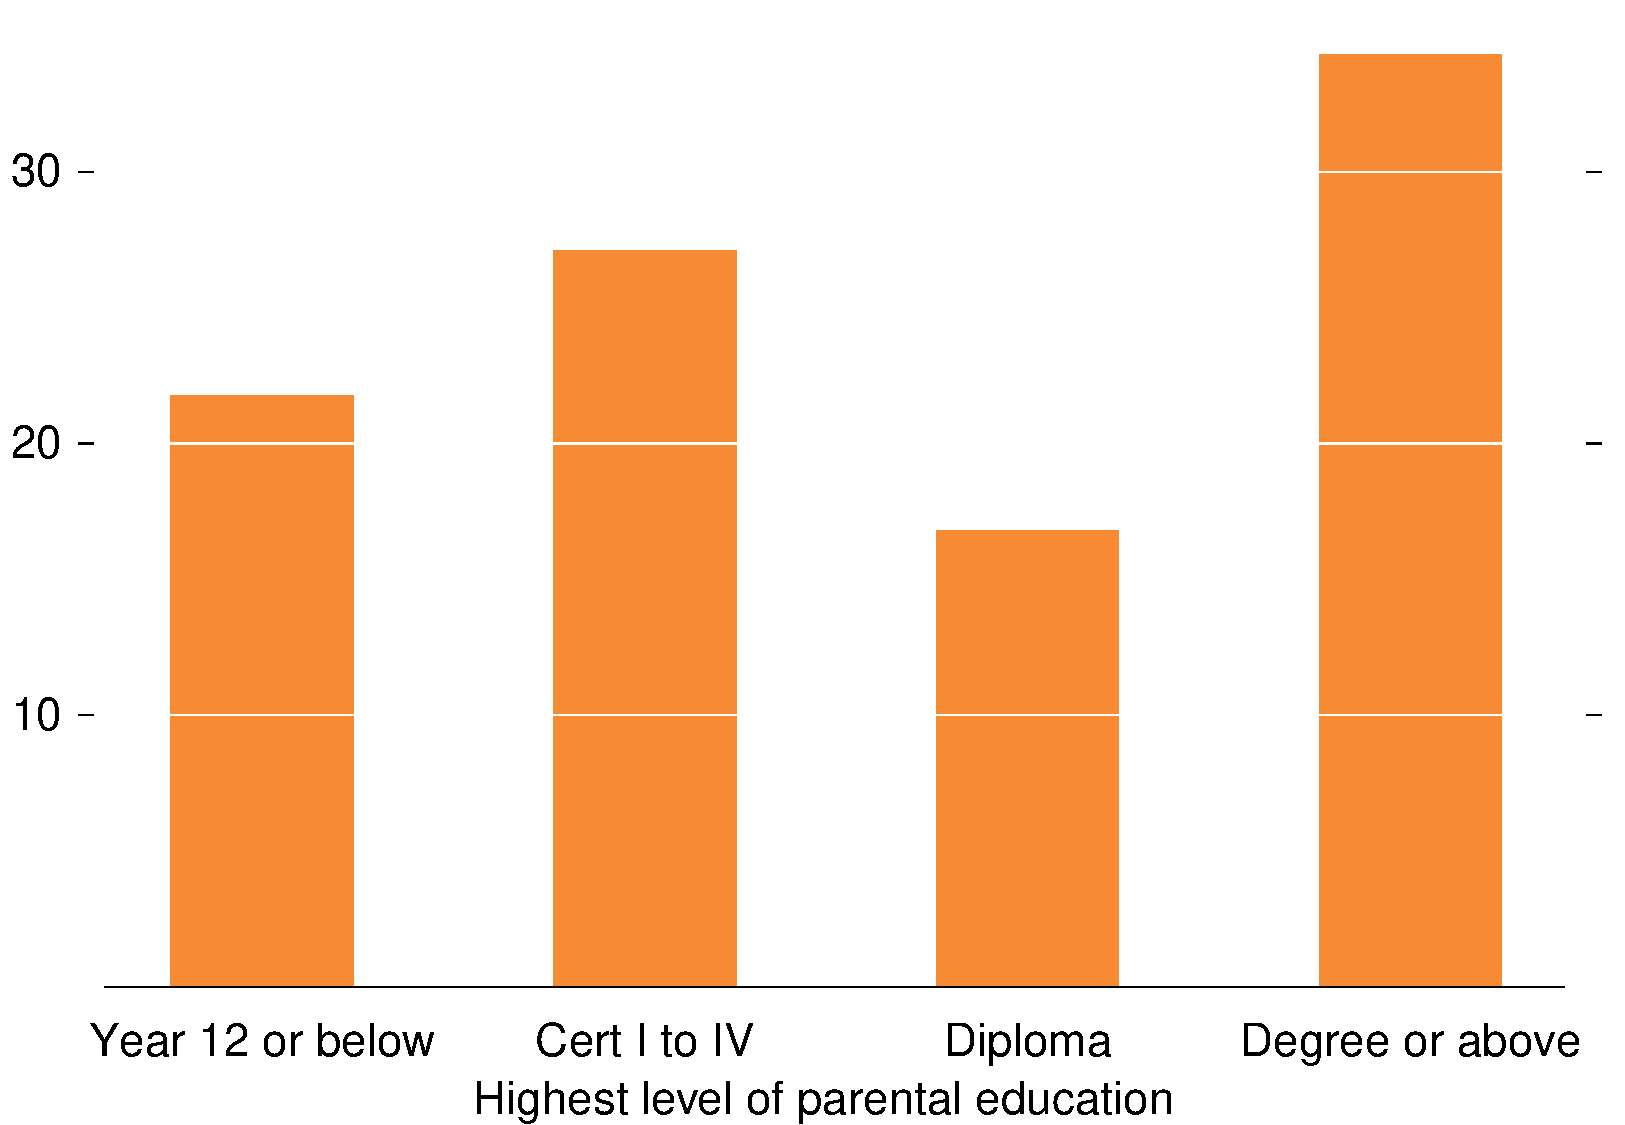
\includegraphics{atlas/Parental_ed.pdf}\label{fig:parental_ed}

\source{Grattan analysis of \textcite{vcaa2015}.}

\notes{Notes go here.}
\end{figure}
\end{frame}


\end{document}